% document style header
\documentclass[a4paper, 12pt]{config/homework}

% import default packages
\usepackage{config/defpackages}
% import custom math commands
\usepackage{config/domath}
\usepackage{pdfpages}

% end preamble
\begin{document}

% document title
\noindent
\begin{tabularx}{\textwidth}{>{\centering\arraybackslash}X>{\centering\arraybackslash}X>{\centering\arraybackslash}X}
Calvin Sprouse & PHYS489 2C & 2024 February 10\\
\midrule
\end{tabularx}

% homework problems begin
% Select and write a reflection on a graded artifact (e.g. homework assignment, test, report) from an upper division physics class of your choice demonstrating that you have met the learning outcome of applying analytical techniques to solve physics and physics-related problems. The application of analytical skills in physics involves implementing mathematical methods to extract insight from a model of a physical system.

% Scan your selected artifact(s) and combine these into a single PDF document.
% Prepare a 1/2 page reflection on how the artifact demonstrates your progress to meeting this goal.
% Upload both pdf documents to Canvas by 11:59pm Friday, February 9.

My chosen artifact for this goal is homework assignment 4 from PHYS451 Analytical Mechanics 2\footnote{Need I say more? Yes.}. This was my second attempt at the homework for which I got a 39/40. On this first attempt I had neglected the very nice notation for central force problems opting instead for a far more complicated analysis of problem 1. My first solution was in more absolute coordinates and lacked an insightful interpretation. I was fortunate to have submitted the homework early and received the feedback in time to correct my solution prior to the deadline. My second attempt, using central forces, yielded the very insightful solution that the system as a whole falls like a single solid object on Earth; that is, it accelerates downwards at \(g\). The spring element of the system then \textit{predictably} introduces a simple harmonic oscillation of the masses independent of their falling! I feel here the power of analytical methods clicked through brute force. With the right technique a solution can be reached that allows a deep understanding of the system in terms of simpler systems. The remainder of the assignment is dedicated to orbital type problems which as an astronomy minor I found quite enjoyable.

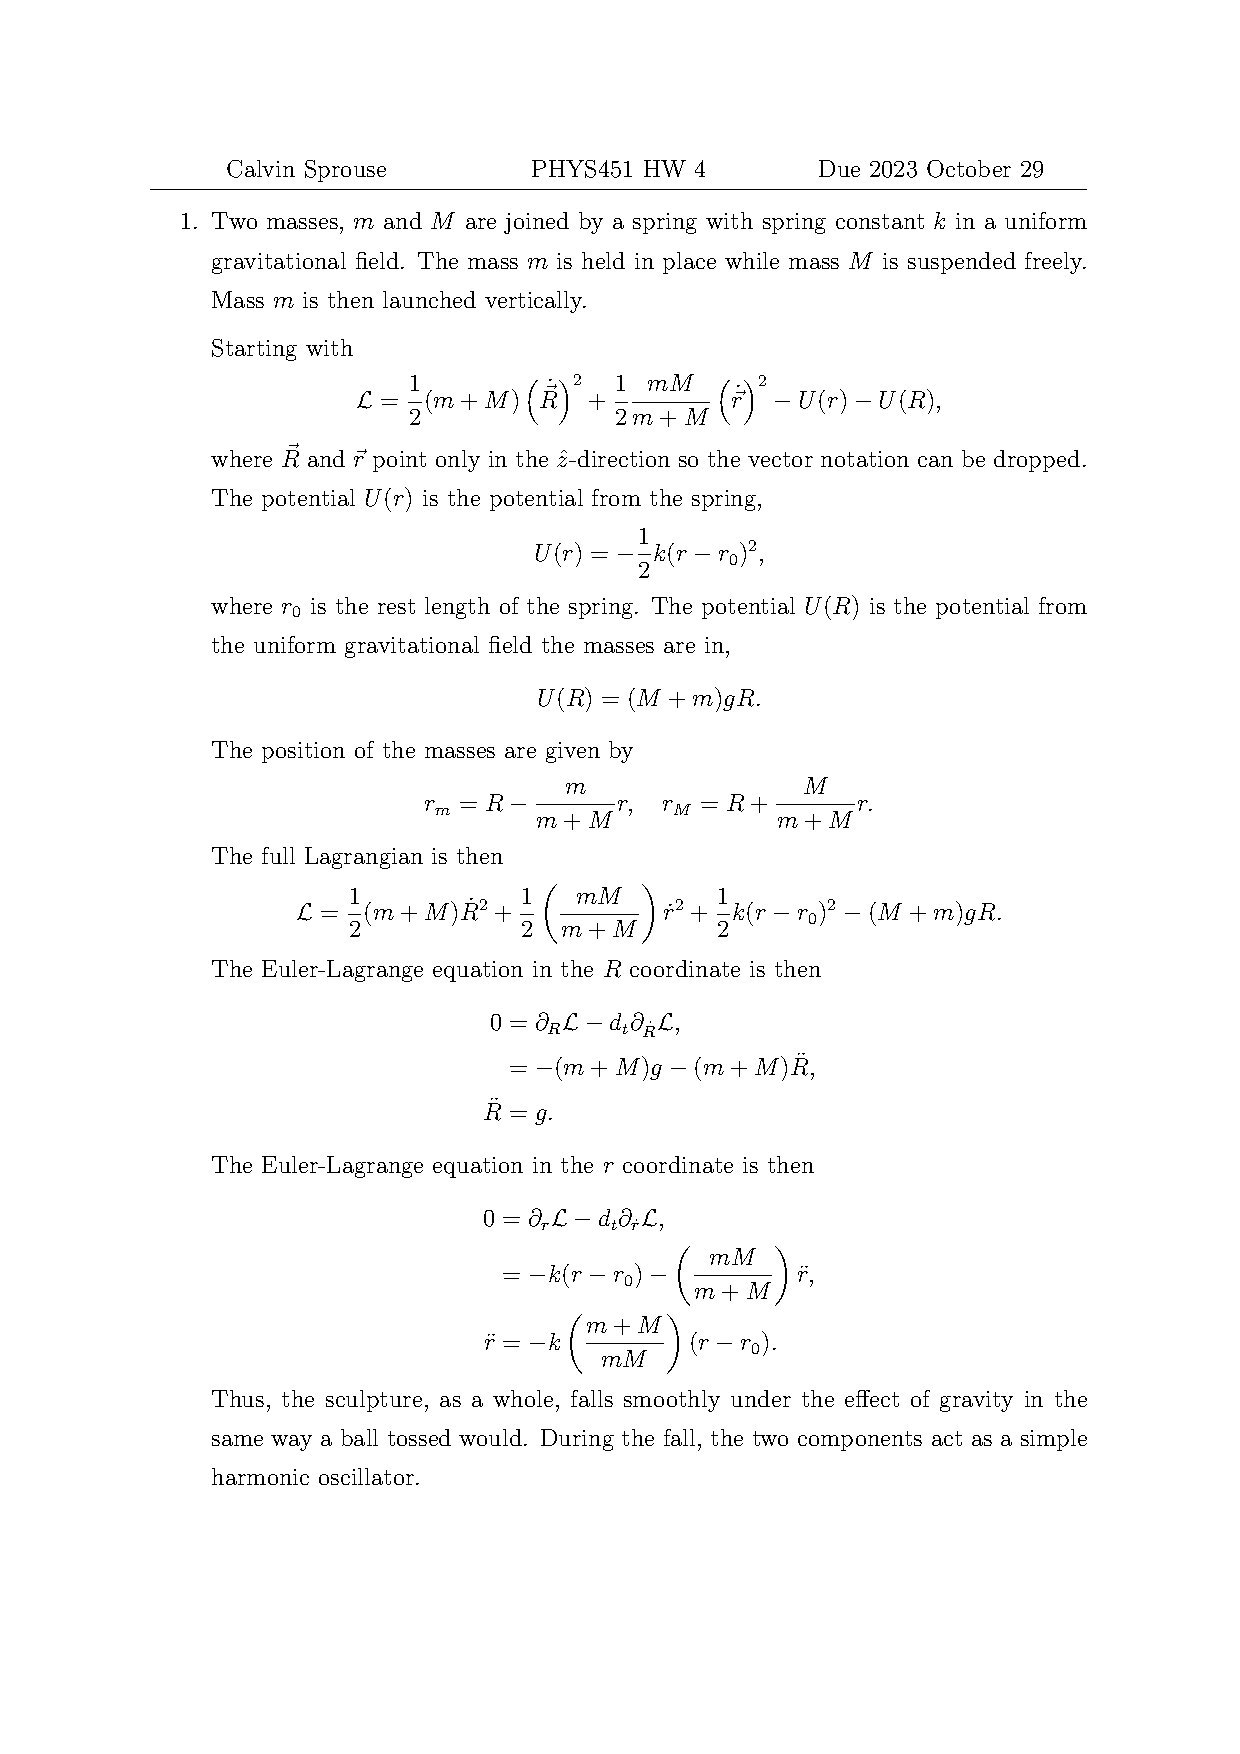
\includepdf[pages=-]{analmech_hw4-1.pdf}

\end{document}
